\documentclass[conference]{IEEEtran}
\IEEEoverridecommandlockouts
% The preceding line is only needed to identify funding in the first footnote. If that is unneeded, please comment it out.
\usepackage{cite}
\usepackage{amsmath,amssymb,amsfonts}
\usepackage{algorithmic}
\usepackage{graphicx}
\usepackage{textcomp}
\usepackage{xcolor}
\usepackage{booktabs}
\usepackage{url}
\usepackage[bottom]{footmisc}
\graphicspath{{./media/}}
\def\BibTeX{{\rm B\kern-.05em{\sc i\kern-.025em b}\kern-.08em
  T\kern-.1667em\lower.7ex\hbox{E}\kern-.125emX}}
\begin{document}

\title{Identification and Measurement of Hierarchical Layout Patterns on User Experience\\
}

\author{\IEEEauthorblockN{Roman Sorin}
\IEEEauthorblockA{roman@romansorin.com}}

\maketitle

\begin{abstract}
TBD
\end{abstract}

\begin{IEEEkeywords}
TBD
\end{IEEEkeywords}

\section{Introduction}
User experience (UX) has continually developed in the field of software engineering and is seen as being highly integral to the success and usability of an application \cite{10.1016/j.jvlc.2017.08.004}. Alongside concepts such as accessibility and presence of I18n in interfaces, perceived user experiences—notable traits such as design, animation, and usability—are one of the most important aspects to consider in the development and analysis of interactions \cite{benchmarking}. Seen both within and beyond software, reputable products and services are known to utilize effective user experience in creating a product that attracts and retains consumers, subsequently expanding the product influence. User experience drives both offline and online interactions that result in psychological and economic impact on consumers and businesses. User experience is a broad and highly expansive field that can take the form of layouts; colors; fonts; copy; animations; and more granular aspects of design and interaction, making UX highly complex to assess and properly execute. In this study, the impact which hierarchical layout structure and design patterns have will be of focus to approach user experience in web interfaces from a bottom-up approach and architectural stance, addressing the fundamental integration of components in the presentational layer.

From one perspective, user experience is derived from the physiological interaction between user and system \cite{10.1145/2688203}. As interfaces and applications are developed further to suit the needs of consumers and developers alike, there exists a significant need to address the psychological implications of human-computer interaction in a more focused and detailed pursuit. Conversely, this continual development of products and experiences creates a significant amount of both practical and technical applications for user experience to manifest itself within, providing for new theses and findings. Within the previous decades, several studies have explored the importance of user experience on this success of products and applications \cite{doi:10.1080/07370024.2011.646927, mousetracking, parallax} in various facets. A common pattern that exists in much of the current research on user experience regards the aesthetics and appearance of a website with consideration of both higher and lower-level abstraction. When analyzing judgment and response by users, aesthetic and appearance is a large determinant in utilization and rates of recurrence \cite{10.1145/3206025.3206039}. In the domain of product and application development, the quality of the experience is extremely vital in progressive rates of user retention, user satisfaction, revenues from sales and advertising, and other analytical measures that are used to determine the relative success of a product or application. Of the serious need for appealing and usable interfaces are businesses that rely on online traffic for customers, and identification and use of these interfaces may provide an advantage over the competition; increasing revenue and attraction by customers to the respective site \cite{10.1145/3206025.3206039}. Consequently, definitive data on optimal layouts by use cases can serve as being beneficial to businesses in both financial and social capital. Moreover, synonymous with the DRY \footnote{DRY: Don't Repeat Yourself. A principle aimed to reduce repetition within software designs} and SOLID \footnote{SOLID: Single-responsibility principle, Open-closed principle, Liskov substitution principle, Interface segregation principle, and Dependency inversion principle. SOLID is a mnemonic acronym describing five design principles aimed to improving software designs.} principles used in software engineering for program readability and maintainability, designers may look to these data to optimize their processes and focus on more granular parts of the system; and developers can be more oriented towards releasing minimum viable products with confidence and reasoning for utilizing a given layout.

In this context, hierarchical features describe the components found making up a layout, and a layout may thus be referred to as layout hierarchy.

A major limitation of UX and its applicability is the granularity found within even the foundational layouts, ignoring any higher-level or specific abstractions. Layouts are recursive and cascading, consisting of components which contain a great degree of subjectivity, development, and iterative processes. These iterative processes take a significant amount of time to implement and analyze, relating to the engineering debt that occurs within design and development \cite{4293575}. Considering the complexity of an interface composed of several different components (all of which are recursive and componentized themselves), the difficulty in achieving an optimal layout in terms of UX is quite evident. As such, the fluidity of design is likely a reason behind the lack of data and definition of layouts, despite patterns in layouts being common and each being utilized in thousands of cases. Even as UX expands as a field and significant area of focus within software engineering, research is relatively limited and restricted to case studies and internal data at best, suggesting a need for a method for identifying these data.

There have yet to be studies that provide definite data on how layout hierarchies affect UX metrics, and correspondingly no models are proposed to identify this correlation. Consequently, this study presents two research questions:

\renewcommand{\labelitemi}{$\textendash$}
\begin{itemize}
  \item (1) How does layout hierarchy impact user experience metrics?
  \item (2) In the future, how can hierarchical features best be implemented to optimize overall user experience?
\end{itemize}



This paper proposes an approach/model to find objective data through the use of machine learning models, more specifically K-means clustering \footnote{K-means clustering is an unsupervised machine learning algorithm, which aims to find groups in data, with the number of groups being specified by variable \(K\). Data provided to the K-means algorithm are clustered according to similarity in features.}, and preliminary layout analysis through collection of the highest-indexing sites by a specified region. Further, this paper seeks to identify how user behavior is affected by the most common layout hierarchies/interfaces found by this model, and suggest replication with additional avenues and narrow scopes to further understand the correlation between user experience metrics and hierarchies.

\section{Method}

\subsection{Design}

A paired analytical and experimental approach was taken to identify common layouts, their hierarchy, and potential associations to user behavior. The analytical procedure utilized scripts and applications \cite{sorin_2020} built specifically for this study to query various APIs \cite{antoniou_2015, deepai}, collect screenshots of sites and manipulate/process screenshots for use in K-means clustering and weighted image overlaying. These K-means clusters were then assessed and manually analyzed to identify common patterns in layouts within a cluster, of which an experimental layout was then derived. Experimentally, a web application was built \cite{sorin} to track user interaction with the presented interfaces. A multi-faceted approach was taken to track and analyze user behavior, such as the use of heatmaps and analytics tools. Heatmaps for both eye and mouse movement are both well-known and effective methods of behavior analysis, as it can provide valuable information in the form of click amount, location, and scroll \cite{mousetracking}, and the service "Hotjar" was used for this application \cite{hotjar}. Analytics tools, like "Google Analytics" as used here \cite{google_analytics}, can provide a wide set of information that can assist in the evaluation of behavior; this information includes demographics, page views, session lengths, and navigation patterns. As the participants worked through the experiment, timestamps representing the start and end of their "session" were collected and set in a document storage service provided by Google's Firebase \cite{google_firebase}.

\subsection{Analytical procedure}

In order to determine common layouts across highest-indexing sites, preliminary data in the form of images had to be collected to be used in the clustering algorithm. The analytical process began with queries to an API provided by Amazon Web Services, known as the "Top Sites API", which returns the highest ranking or indexing sites based on traffic and other factors \cite{antoniou_2015}. 1002 sites were returned after the responses to the API were parsed and filtered. The Top Sites API returns highest ranking sites specified by region, and the "global" region was specified to make a more broad initial analysis of common layouts globally. Sites were then tested to ensure that they were accessible and active, as some were no longer active or contained a 500 (server) error at the time of data collection. After requesting a site at its URL, a screenshot in RGB color space was taken.

Due to current applications of optimizing API requests and data loading, a more lengthy approach had to be taken to take an automated screenshot. Three separate issues were identified during the screenshot process: sites that implemented lazy loading, infinite scrolling, and asynchronous calls. In a traditional browsing context, these are not issues and often improve the user experience. However, these three concepts present an issue in automation and thus regular user behavior had to be emulated before taking a screenshot of the site. More specifically, the following restrictions and process was put into effect:

\renewcommand{\labelitemi}{$\textendash$}
\begin{itemize}
\item Screenshot/scroll height was limited to a maximum of 30,000 pixels
\item The web driver initially moved from its current position to the new scroll height every five seconds, up until the maximum was reached
\item Upon reaching the maximum height, the driver jumped to the 0th pixel (height) and rescrolled in increments of 200 pixels every 0.5 seconds
\item After both passes over the page to ensure all content is loaded, a screenshot was then taken.
\end{itemize}

After review, it was seen that this approach was incredibly effective in retrieving usable screenshots that accurately represented the typical content of a page. Figure \ref{fig:rgb} shows an example page collected in RGB color space through the screenshot process.

\begin{figure}[!t]
\centering
\label{fig:rgb}
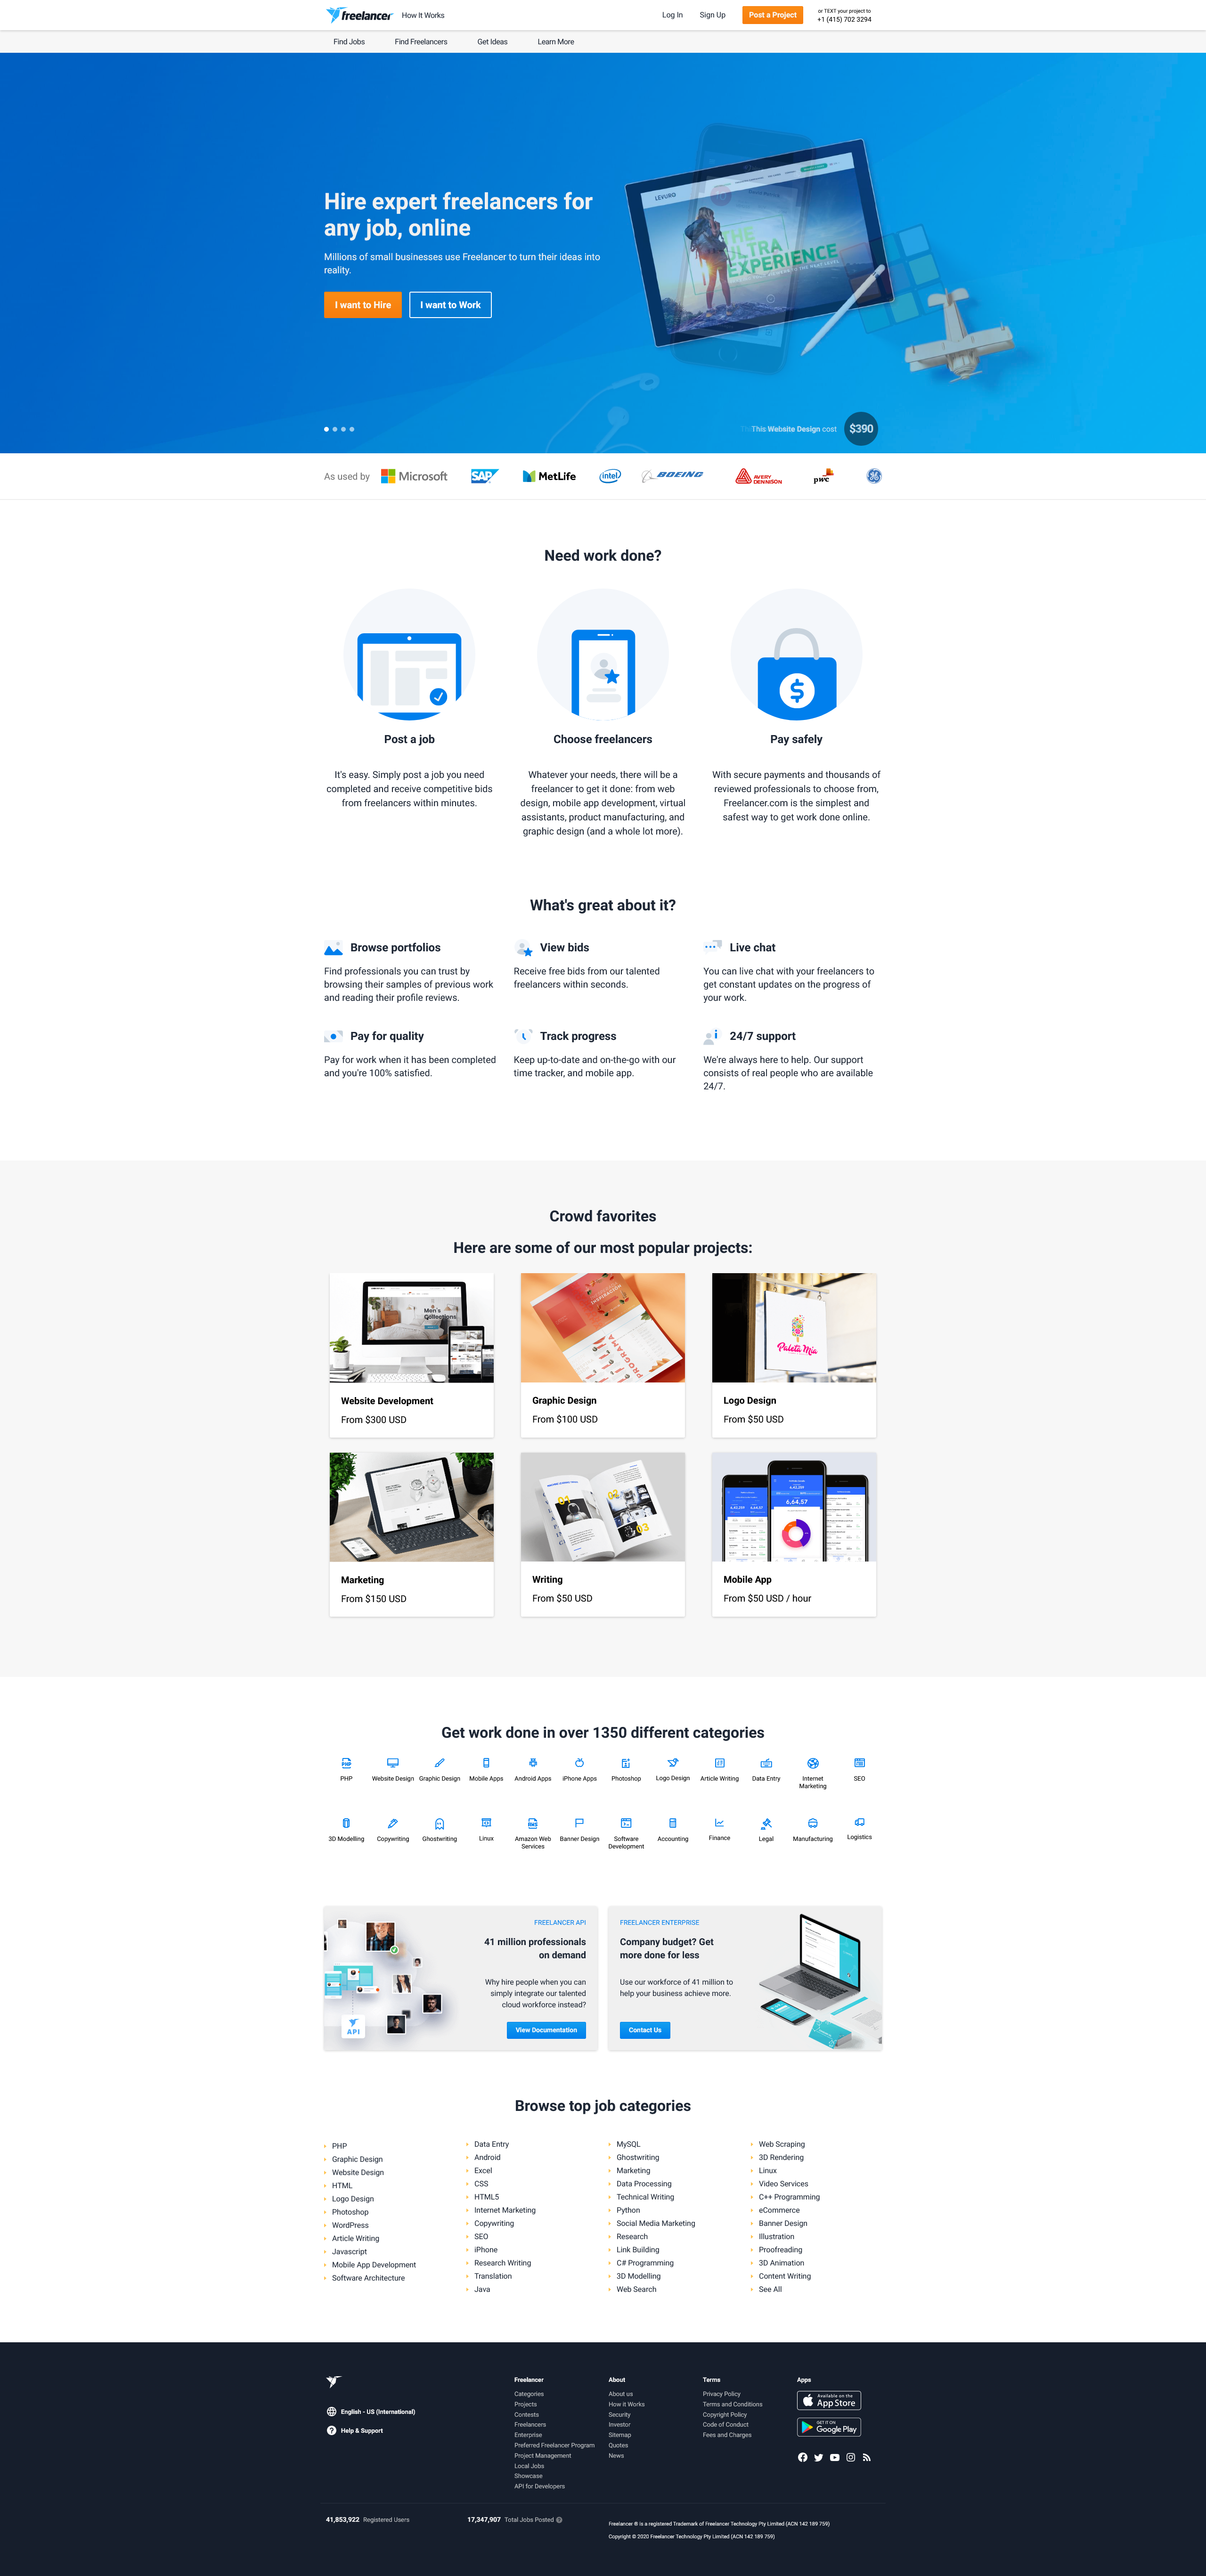
\includegraphics[width=2.5in]{media/freelancer_com_original.png}
\caption{An example output image due to subclustering.}
\end{figure}

After all RGB screenshots were taken, a secondary image processing step was taken: the conversion of all RGB screenshots to greyscale, using the cvtColor function provided by OpenCV \cite{cv2color}. This step was taken to minimize the potential influence that color could have on clustering or similarity, since the focus of clustering was layout hierarchy, not color schemes. 
Screenshots were then reassessed to check that they met the minimum height of 1440px to circumvent technical glitches and potentially invalid array operations. Images below this minimum height were removed, and widths always remained constant (2560px) due to being taken on a single device. Following setting a minimum height, the remaining images were iterated over, and a flag variable of 50,000 px was set. This flag variable was then set to image heights that were less than this dimension, which eventually found the absolute minimum height. All images were then cropped using OpenCV to this minimum height to ensure all image dimensions were equal. Figure \ref{fig:greyscale} shows the previous screenshot (figure \ref{fig:rgb}) after being processed and normalized for clustering.


\begin{figure}[!t]
\centering
\label{fig:greyscale}

\includegraphics[width=2.5in]{media/freelancer_com_processed.png}
\caption{An example output image due to subclustering.}
\end{figure}

In the initial data collection, it was observed that responses had returned sites with the same root domain, but also may have differed by subdomain, organizational TLD (top-level domain), and geographical TLD. For reference, a domain is structured in the format of

\begin{equation}
    [subdomain].domain.tld.[geo]
\end{equation}


These differing sites could not be automatically eliminated due to potentially serving different purposes: a subdomain may map to a dashboard application, another subdomain handles support and status pages. Geographic modifiers, such as .ca or .uk also might not affect content, but rather make the application available to different regions. Because he goal of the analysis was to provide unique data for the K-means model to cluster, rather than providing many of the same sites, another process was established for determining the uniqueness of a page's content between root domains and subdomains:

\renewcommand{\labelitemi}{$\textendash$}
\begin{itemize}
\item Explode all URLs, replacing the period delimiter with a hyphen instead; take a note of the "count" to determine what the root URL is, and what the subdomain/TLDs are
\item Filtered domains were sorted using insertion sort to identify base domain and duplicates.
\item Make an API request to an image similarity API provided by DeepAI \cite{deepai} containing the two source images
\item If the threshold value is above the set maximum, remove the lower ranking site and instead keep the URL with higher ranking precedence
\end{itemize}

A threshold of 15 was set through trial-and-error, and comparisons between made between greyscale images to ensure that color space was, once again, not a factor in determining unique content. After ensuring that all screenshots could be considered "unique" content, these images were then fed into a Keras VGG16 pretrained model \cite{simonyan2014deep} to perform K-means clustering algorithm with K = 4 clusters selected. Due to some clusters containing several hundred images, an image overlaying function was run inside of each cluster to generate sub-clusters of maximum 50 images each. sub-clusters were displayed as a PNG, where the denser parts of the image (greyscale, overlay weighted 50/50) represented the common features in layouts. These features were then manually extracted and represented in a mockup. After each cluster had mockups generated, mockups were analyzed and some features were detracted from the mockup due to overlapping features/clarity of the layout. Three common layouts could be realistically created and identified, and mockups were then converted into web components with TailwindUI \cite{tailwindui}.

\subsection{Experimental procedure}

The experimental portion of the study was conducted through a web application built to host the experiment and information related to the experiment \cite{sorin}. As seen in figure \ref{fig:landing}, upon loading the site, participants were presented with a message describing the entire study in brief, directions for participation, and information on what data is collected and how it will be used. Consent was provided by the participant providing their email and then pressing "begin"; no data were collected up to this point. After pressing "begin", the participant was randomly assigned to a layout (interface) and could not assign themselves to another interface. In the directions, participants were instructed to navigate through the interface and identify how to begin using the product either through registration or purchase, and to emulate their typical behavior when they use a real-world application. Each interface contained at least one "call-to-action" section, and at least one "target", which was essentially a button or link that would theoretically allow a user to register for or purchase a product. After pressing a target, the participants were then redirected to the final screen confirming that their participation in the experiment was finished.


\subsection{Participants}

This study's participants voluntarily participated in the experimental portion of layout analysis. Individuals were age 18 and older, with all participants being from the United States. All participants were expected to have familiarity and experience with navigating layouts and websites, and several individuals had several years of work experience in software engineering and computer science fields. No compensation or reimbursement was provided for involvement in the study. All participants successfully completed the experiment. Participants were recruited through direct and indirect advertisement/sharing of the study. Participation was limited to devices with a minimum screen width of 1024px or a large breakpoint, as only desktop-based layout interfaces were presented. After the experiment, participants were thanked and then provided with an email for further inquiries.

\section{Results}

This section presents the results of both portions of the study, including the numbers of sites throughout processing stages, number of clusters and sites within each cluster, and the observed behaviors of users based on session lengths. Overall, it was shown that there was a minimal variance of the session lengths in the layouts as they compare to each other, and that layout did not affect a user's ability to complete the task as it relates to time.

\subsection{Clustering}

Following the collection of data from the Top Sites API \cite{antoniou_2015}, the data sets were run through the image processing and filtering stages. To simulate the importance of this processing stage as is relates to the use of data, Table 1 {stage-table} shows the number of sites used in the analytical portion of the experiment as it relates to each stage. In stage 0, which is initial data collection and parsing of the API, 1002 sites were returned. Stage 1 concerns the removal of inaccessible and inactive sites as the application collected screenshots of each site, resulting in 975 sites being left for processing. Stage 2 concerns the comparison of the same root domain sites using the image similarity API \cite{deepai} and an arbitrarily set threshold of 15, eliminating subdomains and TLDs with content that too closely resembled that of the higher ranking domain. In addition to similarity processing, reshaping of the resulting screenshots led to those which did not exceed the minimum height of 1440px to be removed, reducing the sample size to 863 sites. These remaining screenshots were deemed unique and fit the minimum dimensions after being converted into a two-dimensional array enough to be clustered using the K-means algorithm.


\begin{table}[]
\caption{}
\label{tab:my-table}
\begin{tabular}{@{}l|lll@{}}
\toprule
Stage & 0    & 1   & 2   \\
n     & 1002 & 975 & 863 \\ \bottomrule
\end{tabular}
\end{table}

Due to a lack of appropriately typed data to apply either the elbow method \cite{elbow} or gap method \cite{gap} to identify the optimal number of clusters to be used in K-means, an arbitrary but reasonable value of 4 was selected, outputting four groups of clustered (similar) images. This K value of 4 was most reasonable for simplicity and ease of evaluation. Table 2 {cluster-table} illustrates the number of images per cluster after running the K-means model, where cluster 0 had n = 242 images; cluster 1 had n = 125 images; cluster 2 had n = 111 images; cluster 3 had n = 385 images. To ease the manual analysis of cluster results, such as in the case of cluster 3, cluster results were iterated over and a weighted image was generated for every 50 images, defining a "sub-cluster". Images within a sub-cluster were blended using the OpenCV addWeighted function \cite{cv2addweighted}.

Table {cluster-table} illustrates the number of sub-clusters per cluster, with cluster 0 having 5; cluster 1 having 3; cluster 2 having 3; cluster 3 having 8. Figure \ref{fig:subcluster} shows an example sub-cluster from a given cluster to better illustrate the intention and output of the weighted images and its improvement on clarity for analysis.

\begin{table}[]
\caption{The number of sites and sub-clusters per K-means cluster group.}
\label{tab:my-table}
\begin{tabular}{@{}lll@{}}
\toprule
Cluster & n  & sub-clusters \\ \midrule
0    & 242 & 5      \\
1    & 125 & 3      \\
2    & 111 & 3      \\
3    & 385 & 8      \\ \bottomrule
Total & 863 & 19     \\ \bottomrule
\end{tabular}
\end{table}

\begin{figure}[!t]
\centering
\label{fig:subcluster}
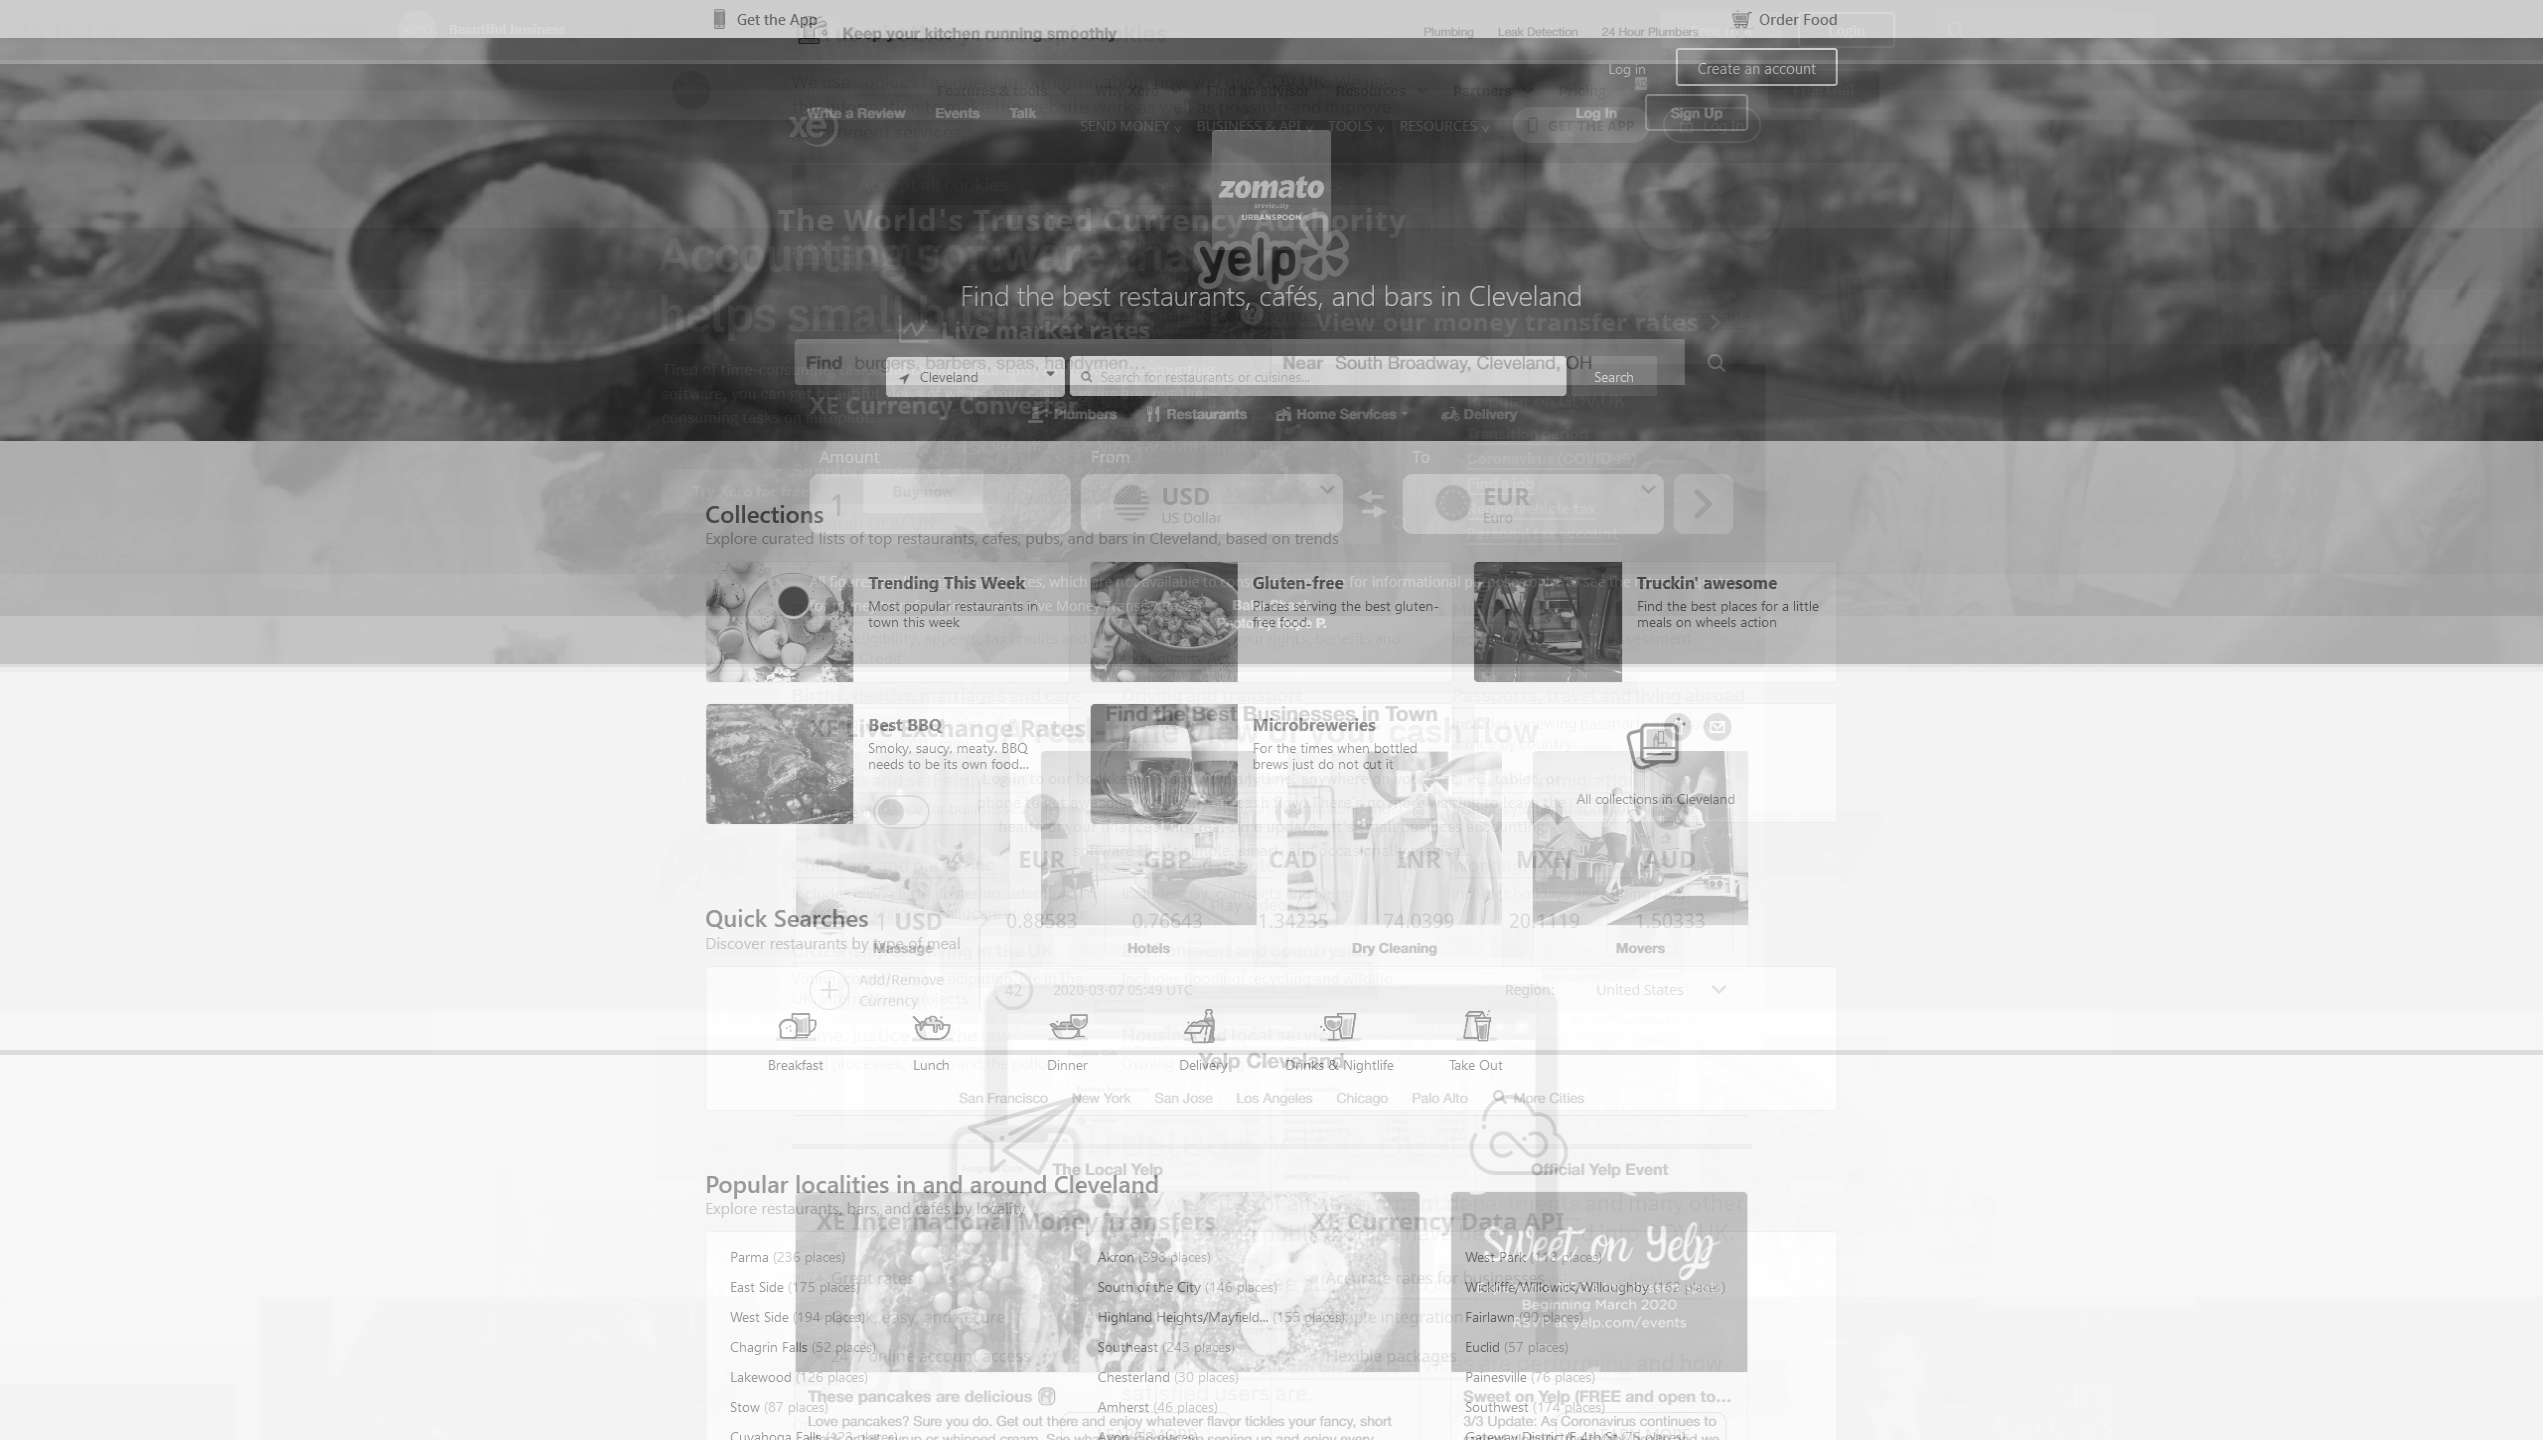
\includegraphics[width=2.5in]{media/subcluster2.png}
\caption{An example output image due to subclustering.}
\end{figure}


Within sub-clusters, common features could be identified based on image/pixel density (i.e., the darker portions of an image or where objects are clearly overlapping) to create one layout per cluster. Due to a lack of obvious variance between two of the four layouts created, the number of layouts was reduced from 4 to 3 to better represent differences in layout hierarchy for implementation. Figures \ref{fig:variant0}, \ref{fig:variant1}, and \ref{fig:variant2} show the layouts that were implemented in the experimental portion of the study.

Qualitatively, these layouts mostly differ in the hierarchy or placement of components relevant to this study, such as the call-to-action and targets. Figure \ref{fig:variant0} (variant 0) displays an immediate headline, and both the call-to-action and targets (3) about a third into the interface, with the rest of the content describing features or other product related information such as blog posts. Figure \ref{fig:variant1} (variant 1) immediately displays a headline followed by product features/information. In order to access the call-to-action and target (1), the user has to scroll past at least 50\% of page content; more product related information follows this midpoint. Figure \ref{fig:variant2} (variant 2) has an immediate call to action and target, with product related information and another target following. Variant 2 is the shortest interface and most immediate in presenting information relevant to the task.

\begin{figure}[h]
\centering
\label{fig:variant0}
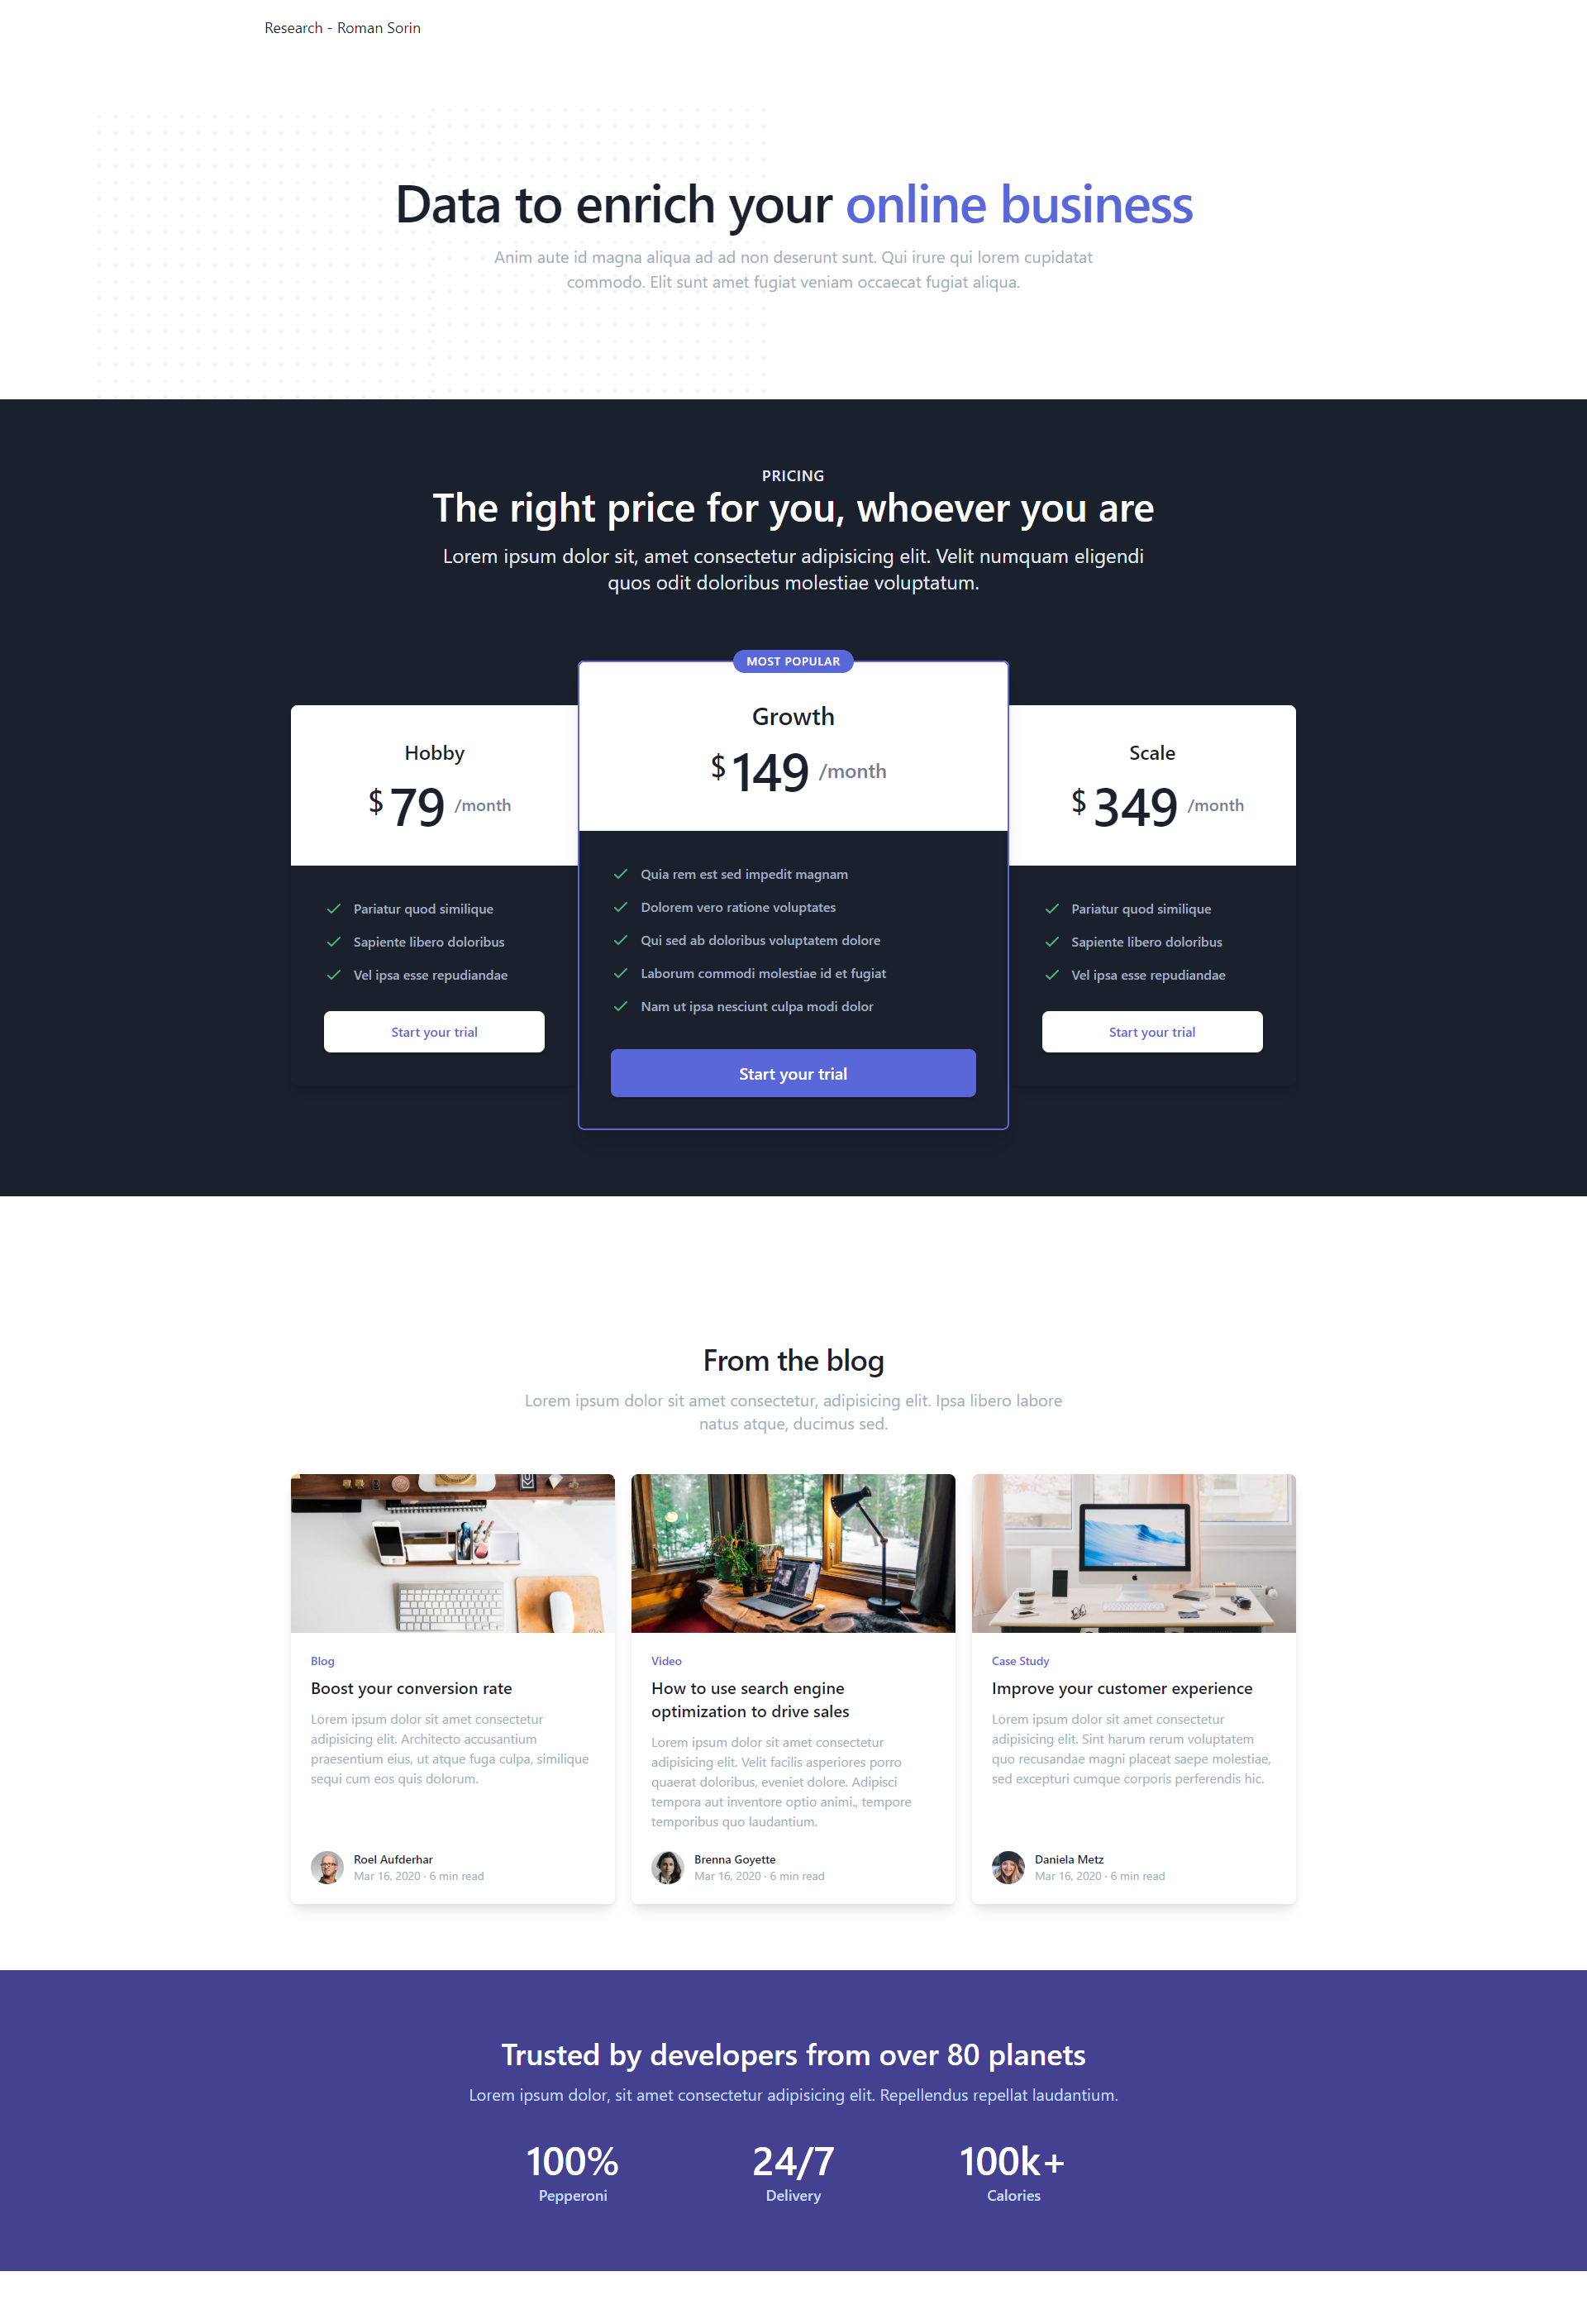
\includegraphics[width=2.5in]{media/8nqXhdl3JD8u.png}
\caption{An example output image due to subclustering.}
\end{figure}

\begin{figure}[h]
\centering
\label{fig:variant1}
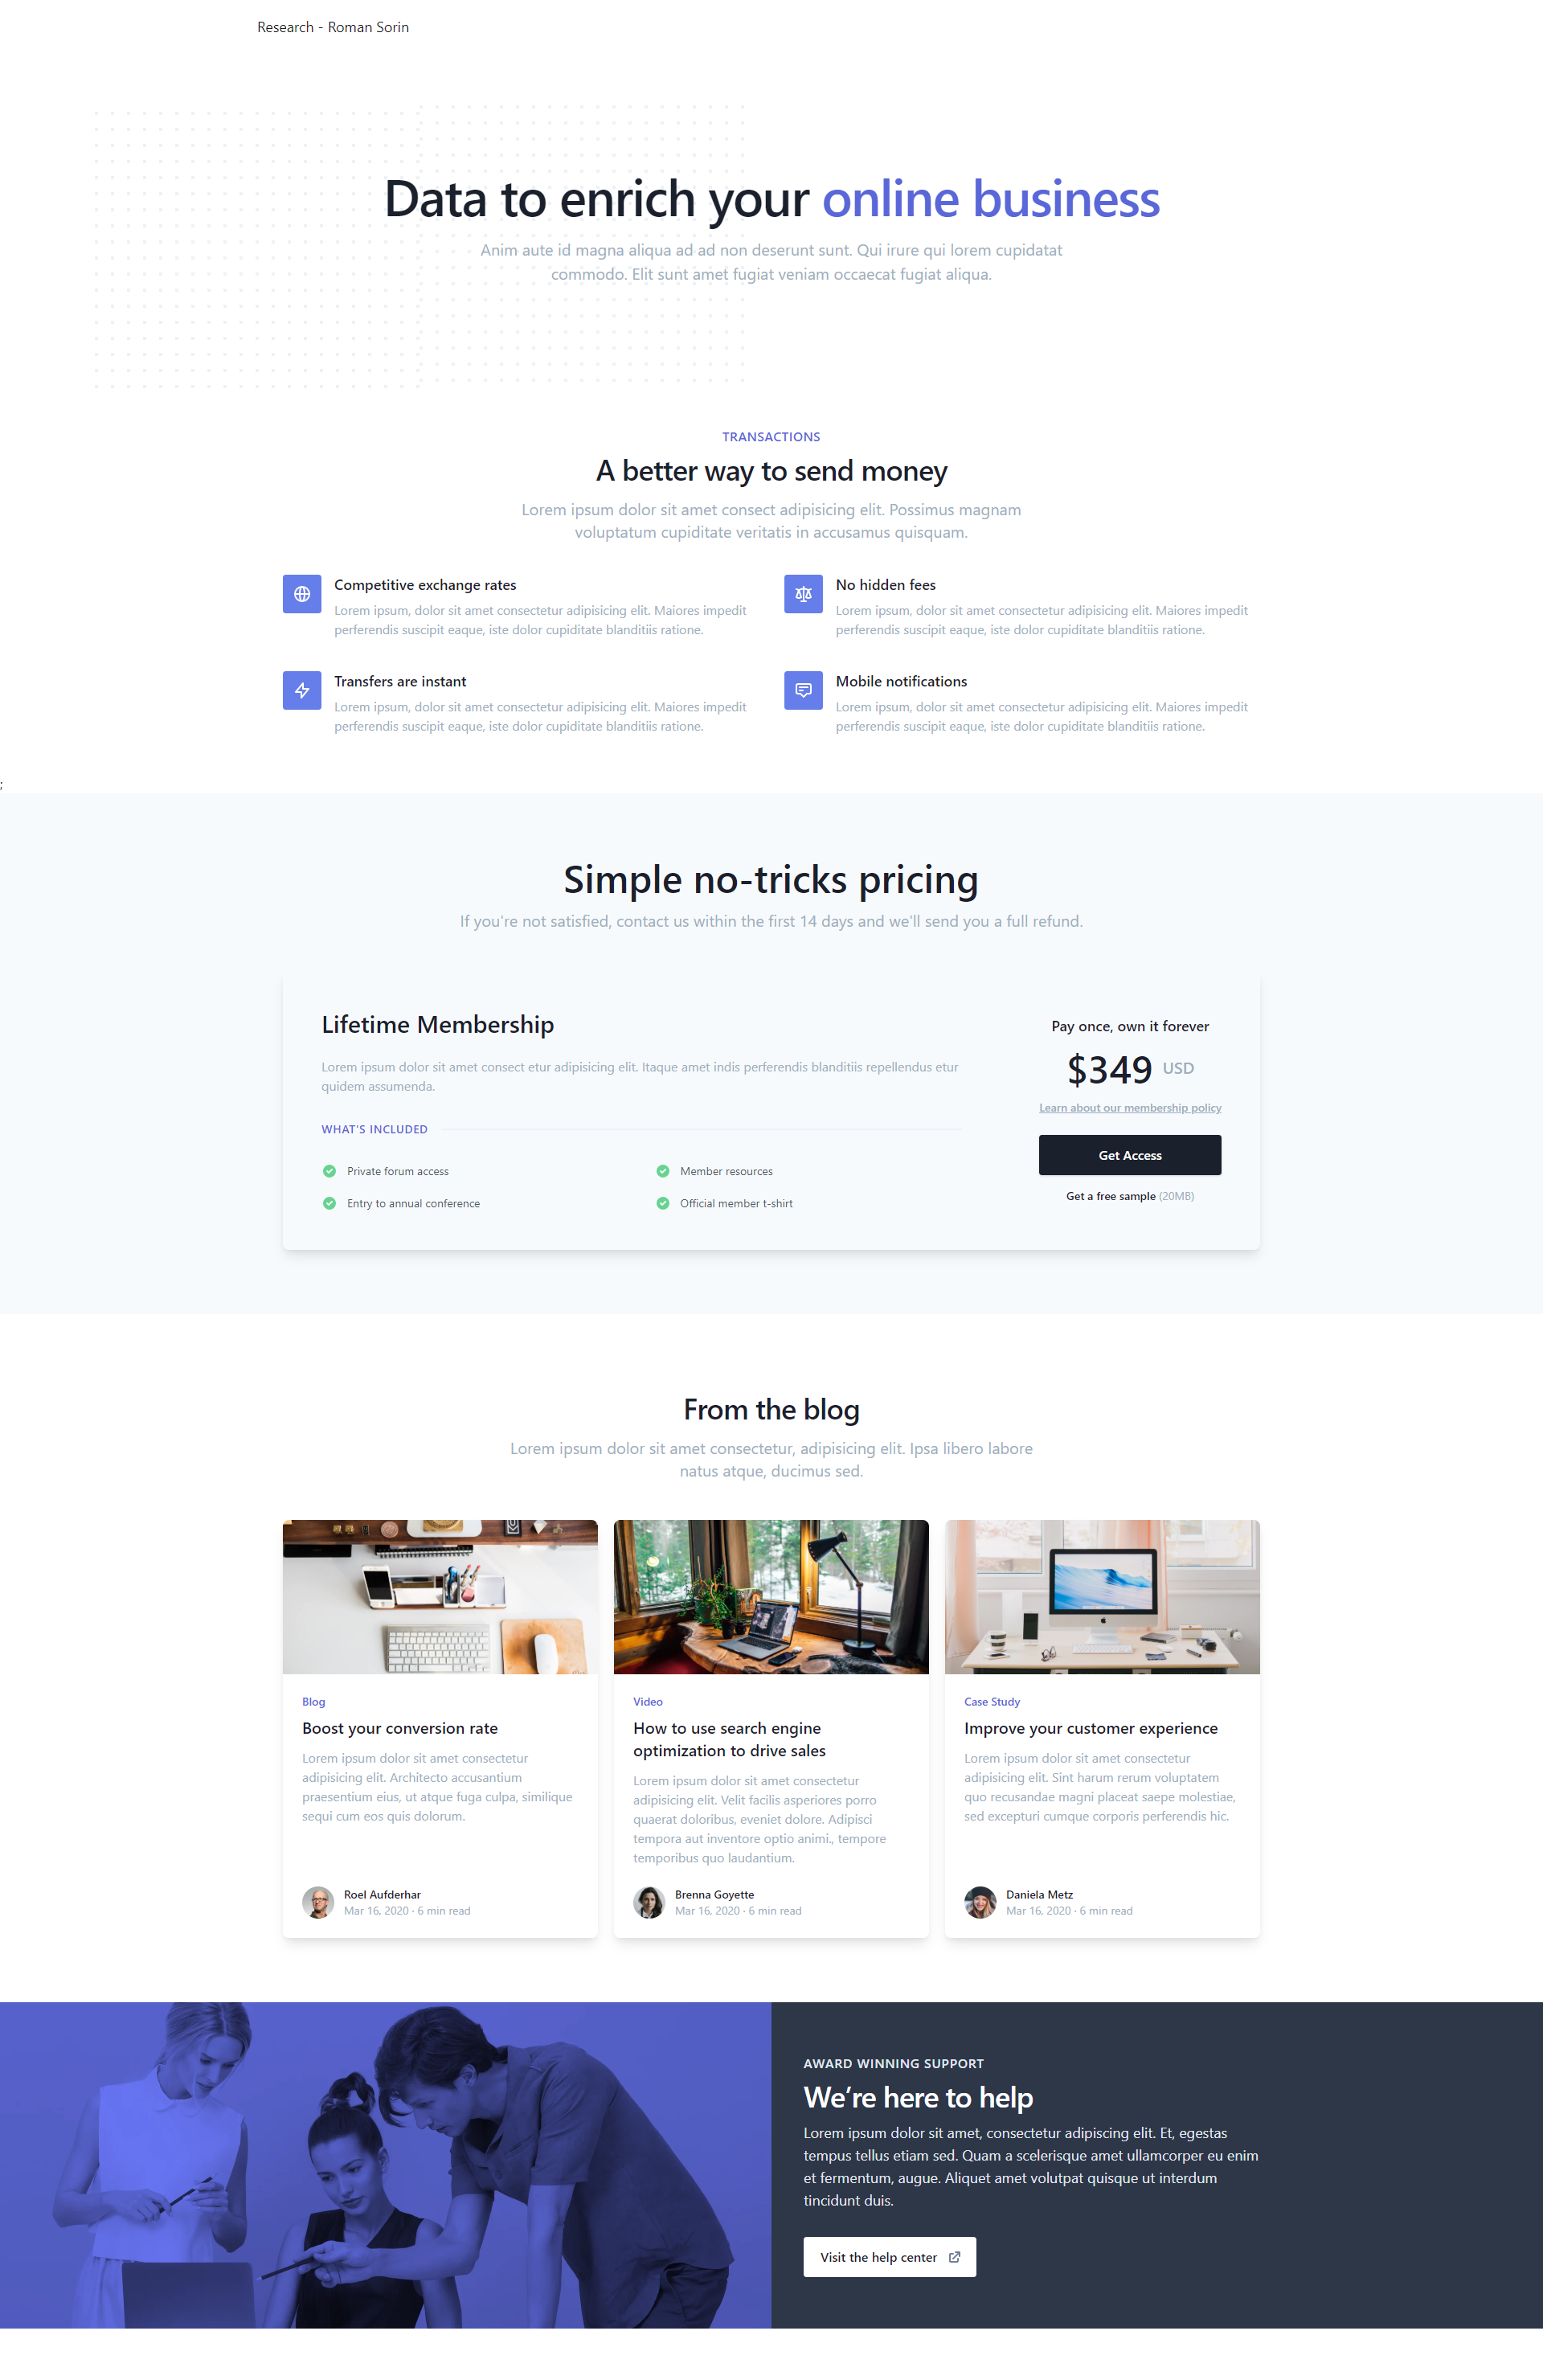
\includegraphics[width=2.5in]{media/hwVB0eKUehxy.png}
\caption{An example output image due to subclustering.}
\end{figure}

\begin{figure}[h]
\centering
\label{fig:variant2}

\includegraphics[width=2.5in]{media/vtc5qYP2r8Ut.png}
\caption{An example output image due to subclustering.}
\end{figure}

\subsection{Implementation}

Though heatmaps and other tracking tools were installed on the experimental site, a technical error led to failure to collect that data and thus only led to session length being collected. Table 3 {variant-length-table} shows a total of 57 data points, with session length elapsed associated with variants. Based on mathematical calculation, two outliers were identified: a value of 80 for variant 0 and a value of 107 for variant 1. These two outliers do not have clear explanations, as factors such as internet connection and someone's understanding of the task could not be assessed/tracked/considered with this implementation. These outliers were not used for following ANOVA testing and variant descriptive statistics, reducing the sample size to 55.

\begin{table}[]
\caption{Data points referring to session lengths recorded for each variant, in seconds.}
\label{tab:my-table}
\begin{tabular}{@{}llll@{}}
\toprule
Variant & 0    & 1    & 2   \\ \midrule
    & \multicolumn{3}{l}{Seconds} \\ \cmidrule(l){2-4} 
    & 7    & 12    & 40   \\
    & 5    & 45    & 37   \\
    & 3    & 3    & 6   \\
    & 60   & 5    & 38   \\
    & 59   & 9    & 3   \\
    & 24   & 3    & 37   \\
    & 5    & 19    & 47   \\
    & 55   & 22    & 54   \\
    & 30   & 11    & 37   \\
    & 24   & \B 107   & 10   \\
    & \B 80   & 15    & 17   \\
    & 5    & 35    & 12   \\
    & 3    & 18    & 24   \\
    & 2    & 29    & 4   \\
    & 35   & 43    &    \\
    & 28   & 9    &    \\
    & 15   & 7    &    \\
    & 9    & 12    &    \\
    & 6    & 26    &    \\
    & 18   & 17    &    \\
    & 17   & 38    &    \\
    &     & 33    &    \\ \bottomrule
\end{tabular}
\end{table}

Using a one-way ANOVA statistical test, analysis of the session length associated with three variants showed that the compared interface variances were found to be statistically insignificant at \(p < .10\). Table 4 {descriptive-stats-variants-table} shows descriptive statistics associated with each variant, while table 4 {anova-table} shows information relevant to the ANOVA test. The means of the three treatment groups were found to have a p-value of 0.485862, and an f-ratio value of 0.73194. While the means were relatively similar across treatment groups \((T_1 = 23.33, T_2 = 23.55, T_3 = 26.14)\), the potential effect of the extreme values is unclear unless the test is rerun without the outliers. Table 5 shows additional information relevant to the ANOVA test.

\begin{table}[]
\caption{Descriptive statistics for recorded data points of each variant.}
\label{tab:my-table}
\begin{tabular}{@{}lllllll@{}}
\toprule
   & n & Mean & Min & Max & SD  & Median \\ \midrule
V_0 & 20 & 20.5 & 2  & 60 & 19.00 & 16   \\
V_1 & 21 & 19.57 & 3  & 45 & 13.14 & 17  \\
V_2 & 14 & 26.14 & 3  & 54 & 17.27 & 30.5  \\ \bottomrule
\end{tabular}
\end{table}

\begin{table}[]
\begin{tabular}{@{}lllll@{}}
           & \multicolumn{3}{l}{Treatments} &    \\
           & 1    & 2    & 3    & Total \\
N           & 20    & 21    & 14    & 55  \\
∑X          & 410   & 411   & 366   & 1187 \\
Mean         & 20.50  & 19.57  & 26.14  & 21.58 \\
∑X\textasciicircum{}2 & 15268  & 11495  & 13446  & 40209 \\
SD          & 19.00  & 13.14  & 17.27  & 16.44
\end{tabular}
\end{table}


\begin{table}[]
\begin{tabular}{@{}lllll@{}}
Source       & SS    & df & MS   &       \\
Between-treatments & 399.52  & 2 & 199.76 & F = 0.73194 \\
Within-treatments & 14191.86 & 52 & 272.92 &       \\
Total       & 14591.38 & 54 &    &      
\end{tabular}
\end{table}

Though the resulting session lengths were found to be statistically insignificant, observing graph 1 of session lengths leads to interesting findings. Variant 1 is seen to have more consistently spaced data points with a lower maximum, whereas both variant 0 and variant 2 had clusters — albeit small — on both ends of the graph, exceeding that of variant 1. Relative to variant 1, variants 0 and 2 took anywhere between 1 to 7 seconds longer for several individuals in both cases.
However, this pattern cannot be clearly explained due to various potential factors and without further analysis or manipulation. As seen in figures 2, 3, and 4, variant 1 had fewer "call-to-action" points and required a further scroll distance to reach the target, whereas variants 0 and 2 both had immediately presented "call-to-action" and additional targets. It is unclear whether this is due to friction of the input field on variant 2, color schemes throughout each variant influencing mood, eye fatigue from the previous screen, or the choice of copy in each section.

 
\section{Discussion}

As web applications continue to advance, it becomes more and more imperative to abstract potential approaches and factors that influence the success of products. In particular, this study aims to converge focuses on user interface — such as UX metrics and layout hierarchy — with the potential benefits of mathematical or statistical optimization. The use of data is not a new concept in identifying the success of products and related items within businesses, however, there is yet some metric to describe how layout hierarchy or other factors may potentially influence overall user experience. As such, this paper proposes a potential approach to identifying common layouts and features in a given domain and optimization with subsequent analysis of the effectiveness of layouts. For web interfaces, many confounding variables may be present that impact the length and ease of a user's site usage. This proposed model would do best if applied on a legitimate product or site with more development to analyze how it performs in real world scenarios, and how other known factors may influence ease. 

Though there is statistical insignificance in this data, this model could be used to validate new layouts against common layouts extracted from top sites to determine the effectiveness of the layout. Though not evident without abstraction beyond statistical results, hierarchy may have been influential in the results of this study, and present itself at a greater scale with a higher sample size or different application of this proposal. The "how" and "where" representation of different components and hierarchical features in each variant likely held an influence on the distribution of data, but more research is required to make the exact factors known.

As mentioned before, variant 1 is of particular interest. Despite having a reduced number of successful targets to click and more scroll distance required to complete the task, leading to more time elapsed, data was more consistent and did not broach the upper ends of the distribution like variants 0 and 2 did. This display of results is unexpected: variant 0 had a large section about a fourth of the height into the interface that allowed users to get started with the product, and variant 2 had a direct call-to-action within the initial viewport. Despite variants 0 and 2 being more accessible and intuitively quicker to get started with, more participants were seen to have trouble with these variants — either figuring out how to use them, or turned away by the format and display of information.

\subsection{Limitations}

As with any study, this study suffers from several limitations that may have negatively influenced results. Beginning with analysis (stage 0), it is possible that too global of a site data collection was specified; the globally highest-indexing sites were returned, and not those specific to a given region. Due to cultural differences and availability of engineering, research, and design, different regions have different opinions on design and different standards on how information should be best presented. Future research and retrials of this proposed model should specify a given region, such as the U.S. or Canada. In addition to selecting too large of a ranking range, this initial study was clearly too broad in terms of categories. While the Top Sites API does not provide data based on category of site, a potential solution could be to cross-analyze/join APIs and identify the category based on a single URL. By specifying region and category, responsible parties can better understand how to present information to their target audience by demographic and focus.

A single K-means clustering in stage 2 may not have been a sufficient or best possible approach to identifying commonalities in images. While some basic image processing and filtering was applied, there are likely other ways to process images for the K-means algorithm to better cluster, such as applying hidden layers using a CNN, or potentially training another K-means model. It may be a better approach to instead focus on individual parts of hierarchy within a layout and cluster those, rather than doing full pages: such as the hero, headers, footers, etc. These cluster data can then be combined to identify the "best" layout by working incrementally. Furthermore, common features or objects can be difficult to detect even in sub-clusters of 50 overlayed images. Considering how limited this data set was and the general manual time required to be invested, it would be impractical — or even impossible — to run manual analysis of overlayed images on a data set of 500,000 sites. It is unclear how this paper's approach of "sub-clustering" was or wasn't useful in identifying common features within a cluster, and if it could have been avoided entirely if another model was used alongside the Keras VGG16. For the purpose of clarity and logic in these interfaces, manual analysis likely led to a degree of bias in design and elements, especially since elements had to be recreated from the clusters/sub-clusters (no elements or copy could be directly copied), which means that the researcher's design tendencies may have affected user experience positively or negatively.

Experimentally, the choice of participant demographic and previous exposure to interfaces may have been counterintuituve. While mostly software engineers and web designers were prompted to participate in the study so as to reduce potential confusion in the required task, this study may have overestimated the degree to which the layout or directions would be considered to be confusing. As such, these individuals are already trained to quickly and effectively navigate through layouts and interfaces, which is non-representative of the actual market or target population. However, this also reinforces the need for live implementation of this study's proposed model in real-world applications, and how it can potentially yield descriptive results when put into effect in these environments.

Generally, this study's methods suffered due to a lack of preexisting research to fill in gaps of inquiry and approaches. In several areas, from data collection to image processing to experimentation, this study creates potential methods and procedures for use by the software engineering community in varying aspects. Replication of this study with more time and larger data sets, as well as addressing the aforementioned limitations of querying category and demographic could very potentially yield results that benefit the software engineering and design community as a whole.

\subsection{Future work}

There are several avenues of improvement and future inquiry in both analytical and experimental contexts. It is highly likely that relying strictly on a K-means algorithm and manual analysis of clusters led to misrepresentation of what the most common layouts really are, or that they could have been considerably more detailed than they were in this study. With that in mind, inclusion of other machine learning based methods and models — such as feature and object detection — in addition to more developed clustering models may allow for better understanding what common features exist in layouts, and how they work together to build hierarchically effective layouts.

In addition to simple clustering and image overlays, the presence of features could potentially be represented by "density", which would require a quantitative and empirical metric of its own. This density could describe features on an interface, which could be aided by "contour maps" to illustrate where components are commonly placed as another measure of layout effectiveness. Pairing this proposed model with widely utilized eye and mouse tracking could be incredibly fruitful, and would allow this model to be ran several more times on a greater scale, providing more data to analyze and generate potential correlations from.

With these increased trials, there is potential to describe the results with a quantitative metric, that may be used to predict the effectiveness of a layout as it relates to UX metrics. Implicitly, this research would allow businesses to focus less on A/B variant testing, and instead explain their decisions through a predictive quantitative metric, providing focus on building products whilst optimizing interfaces.

\subsection{Conclusion}
It's important that the methodology proposed within this study is replicated due to its potential benefit to real-world products and the software engineering community. It is also important to recognize that within this context, both qualitative abstract analysis and quantitative statistical testing is required to identify the effectiveness of a layout, and to identify potential factors that may lead to optimization. Informally, both are applied in isolated case studies, but there is yet to be an abundance of research that blends both to improve the quality of interfaces with widely available models and procedures.

\bibliography{references}
\bibliographystyle{./bibliography/IEEEtran}

\end{document}
